\documentclass[journal]{IEEEtran}
\usepackage{cite}
\usepackage[dvips]{graphicx}
\usepackage{hyperref}

\begin{document}
%Continuous group index and dispersion measurements in slow light corrugated waveguides
\title{Optical phase characterization of integrated photonic devices}
\author{J.~Matres,~G.~C.~Ballesteros,~S.~Mas,~A.~Brimont,~P.~Sanchis,~J.~Mart\'i~and~C.~J.~Oton}
%\markboth{IEEE PHOTONICS TECHNOLOGY LETTERS}%
%{Shell \MakeLowercase{\textit{et al.}}: Continuous group index and dispersion measurements in slow light corrugated waveguides}

\maketitle


\begin{abstract}
We propose a relatively simple experimental setup capable of accurately characterizing the optical phase response of an integrated photonic circuit. The setup is based on a phase-noise reduction scheme using an external heterodyne Mazch-Zehnder interferometer. In particular, we characterize the phase response of different silicon photonic components: undercoupled and overcoupled ring resonators, and a corrugated  waveguide.

\end{abstract}

\section{Introduction}
\noindent In the last years, integrated optics has seen a remarkable development thanks to technological advances but also because its recent trend towards standardization.
The main advantage of photonic integrated circuits is that one can build a extremely complex systems with hundreds of components on a very small footprint and at a very low cost per device.
System design usually requires scattering parameters of single components in order to simulate a complex system.
The measurement of these parameters requires the characterization of the phase response of the element.
This is not straightforward, as under normal circumstances phase noise prevents simple interferometric measurements using for example a Mach-Zehnder interferometer (MZI).


Several techniques have been proposed to alleviate phase noise problems in the fringe characterization of the measurement.
However these techniques usually require very precise temperature control, or very fast tuning rates (70~nm/s in \cite{Vanwiggeren2003} and 40~nm/s \cite{Gifford2005}).
Commercial devices sensitive to phase are typically called optical vector network analyzer (OVNA).
These instruments usually employ tunable lasers with tuning speeds of 100-1000~nm/s.
In this work, we present a relatively simple setup which allows accurate and continuous phase response of the system by using an ordinary tunable laser with tuning speeds in the order of few nm/s.
The cancellation of phase noise is carried out by employing a counter-propagating reference beam at fixed wavelength.
This idea was applied in Ref.~\cite{Mas2012} to characterize chromatic dispersion in waveguides with different geometries.
This paper shows that the setup can be used to characterize the phase response of different building blocks, in particular, silicon microring resonators and corrugated waveguides.
In the former, the measurement allowed us to distinguish undercoupling from overcoupling conditions.
In the latter, a detailed plot of the group index of the corrugation can be obtained from a single segment of waveguide without the need of integrated MZIs and fringe spacing calculations.


\section{Experimental setup}
The experimental setup is shown in Fig.~\ref{fig:dispersionSetup}.
It consists of a fiber-based MZI, where each branch has a an acousto-optic modulator (AOM) which acts as a frequency shifter.
The frequency shift applied to each branch is slightly different, in order to make it heterodyne (in our experiment, the difference was 40~kHz), which produces a beating pattern which can be measured with a lock-in amplifier.
The phase of these beatings with respect to the RF generators provides the phase of the system, but this is also affected by thermal phase noise, which can be as high as several radians per second.
This noise would make unfeasible a phase characterization with a laser with tuning speed in the order of few nm/s. To cancel the phase noise, a reference counter-propagating beam at a fixed wavelength was introduced from the opposite end.
This signal produces another beating pattern which can be detected with a second photodiode, amplified, and used as a reference for the lock-in amplifier.
As thermal fluctuations equally affect both beams, they cancel out, and only the wavelength-dependent phase variations are measured.
An optical delay line (ODL) is also introduced in one branch in order to keep the interferometer balanced when different device lengths are measured. 


\begin{figure}[htb]
	\centering
	\includegraphics[width=3.5in]{dispersion3}
	\caption{Optical phase characterization setup. AOM: acousto-optic modulator. Dashed lines are electrical connections. In light green color is the tunable laser whose phase is monitored in the lock-in amplifier. In dark blue is the counter-propagating beam used as a reference in the Lock-in amplifier to compensate thermal fluctuations.}
	\label{fig:dispersionSetup}
\end{figure}


If the building block to characterize is placed in series with other elements, (couplers, connecting waveguides, tapers, etc.) the measurement requires a reference sample with the same elements, but without the component under test (e.g. the corrugated waveguide).
Before each sweep is launched, the MZI must be balanced in order to avoid too steep slopes in the phase dependence on $\omega$.
In addition, it is convenient to set the wavelength of the counter-propagating reference beam, $\omega_0$, approximately in the middle of the sweep in order to get small phase noise.
The reference sweep provides the system response, which must be subtracted from the measurement which includes the component under test. 


Mathematically, the phase dependence obtained with the lock-in, after subtracting the system response, becomes:


\begin{equation}
  \phi(\omega)= \beta_c L_c - \beta_{air} \Delta L_{air} =\phi_{c}(\omega)-\frac{\omega\Delta L_{air}}{c}
  \label{eq:response}
\end{equation}

where $\phi$ is the measured phase, $\phi_{c}$ the phase introduced by the component under test, $\Delta L_{air}$ the extra length introduced in the ODL to balance the MZI with respect to the reference measurement, and $c$ the speed of light in vacuum. It can be demonstrated \cite{Mas2012} that if the component under test has a length $L_{c}$, then the the group index of the component is precisely:

\begin{equation}
  n_{g} = \frac{\Delta L}{L_{c}}
  \label{eq:group_index_pathBalancing}
\end{equation}

The balancing of the MZI is carried out by minimizing the slope of the phase versus wavelength. A slope equal to zero at a certain wavelength corresponds to perfect balancing, so the group index of the component under test can be extracted. Finally, its dependence on wavelength is extracted from its variation versus wavelength when the sweep is acquired (Section \ref{sec:newTechnique}).

It is worth mentioning that as the lock-in can simultaneously provide the phase and the amplitude of the output, a complete phase and amplitude characterization is possible with the setup in one single sweep. Moreover, amplitude noise due to gradual slight misalignments can also be canceled out by normalizing with the amplitude of the reference signal.


\section{Fabrication}
Samples were fabricated using the EPIXFAB platform, processed from SOI wafers with 220~nm Si thickness, patterned with deep-UV lithography and covered with silica after the etching process. They included ring resonators (section~\ref{sec:ringResonators}) and corrugated waveguides (section~\ref{sec:corrWaveguides}).


\section {Ring resonators}
\label{sec:ringResonators}
Ring resonators are very useful components for filtering, multiplexing, switching and modulating. The most important parameters of the rings are the free spectral range (FSR), the extinction ratio (ER), and the width of the resonance (FWHM), related to the quality factor (Q) and finesse of the resonance ($F$). These parameters depend not only in design but also manufacturing tolerances.

\begin{equation}
	FSR=\frac{\lambda_{res}^2}{n_gL}
	\label{eq:FSRanillo}
\end{equation} 

\begin{equation}
	Q=mF=m\frac{FSR}{FWHM}
\end{equation} 


The transmission equation of a ring can be easily obtained:

\begin{equation}
	E_{out}/E_{in}=\frac{t-A}{1-tA}
\label{eq:transmissionRing}
\end{equation}

Where $A=\alpha e^{j\phi}$, in resonance, is equal to the propagation losses inside the ring ($\alpha$) because $\phi=\beta L= 0,2\pi,4\pi\ldots$


Depending on the relation between the coupling coefficient and the losses, a ring resonator can be:

\begin{itemize}
 \item \textbf{Critically coupled ($t=A$):}  there is no transmission as equation~\ref{eq:transmissionRing} goes to zero.
 The same energy that goes through the coupler exits the ring after multiple turns, the $\pi$ phase shift to enter and exit the ring causes a complete destructive interference at the output.
 
 \item \textbf{Under-coupled ($k<A,t>A$):}  more energy goes through the coupler than inside the ring. So resonances produce small phase and amplitude changes.		
 
 \item \textbf{Over-coupled ($k>A,t<A$):}  more energy goes inside the ring than through the coupler. Each of the resonances causes $2\pi$ phase shift when sweeping the wavelength.
%  Before entering the resonant regime light goes through the coupler and not into the ring (0 rad phase shift), with the ring in resonance most of the energy goes in and out of the ring, with a phase shift of $\pi$ rad.
%  Finally, when leaving the resonant regime, another $\pi$ rad phase shift is produced.
\end{itemize}



\begin{figure}[htb]
    \centering
    \includegraphics[width=3.5in]{ringTesis}
    \caption{Amplitude (top) and phase (bottom) simulations of a 20~$\mu$m ring resonator for different coupling conditions. Notice that only monitoring the phase we can distinguish under-coupled and over-coupled rings.}
    \label{fig:ringDifferentCoupling}
\end{figure}

In paper \cite{McKinnon2009} a method is developed for extracting the coupling and loss coefficients. However the formulas used do not distinguish which coefficient is loss and which is coupling. As we can see in Fig.~\ref{fig:ringDifferentCoupling} monitoring the phase we clearly distinguish an under-coupled ring from an over-coupled, even when the transmission response is exactly the same. 



\begin{figure}[htb]
    \centering
    \includegraphics[width=3in]{r20g250_2}
    \caption{Ring resonator SEM image.}
    \label{fig:semRingPaperRings}
\end{figure}


%\subsection{Phase measurements in ring resonators}
%First we characterized the amplitude response of the rings sweeping the wavelength of a tunable laser at the input and monitoring the output power with a power meter. Then, using setup shown in Fig.~\ref{fig:dispersionSetup} we monitored the phase evolution in the same wavelength range. Finally, 


Amplitude and phase responses were normalized by a waveguide without ring, combined and fitted to the ring transfer function:

\begin{equation}
	H(\omega)=E_{in}/E_{out}=\mathrm{amplitude}\cdot e^{j\cdot \mathrm{phase}} = \frac{t-A}{1-tA}
\end{equation}
 

As we can see in Fig.~\ref{fig:undercoupled} we clearly see that under-coupled rings accumulate $2\pi$ phase shifts while over-coupled have phase rebounds in each resonance as in Fig.~\ref{fig:overcoupled}. 

     
\begin{figure}[htb]
  \centerline{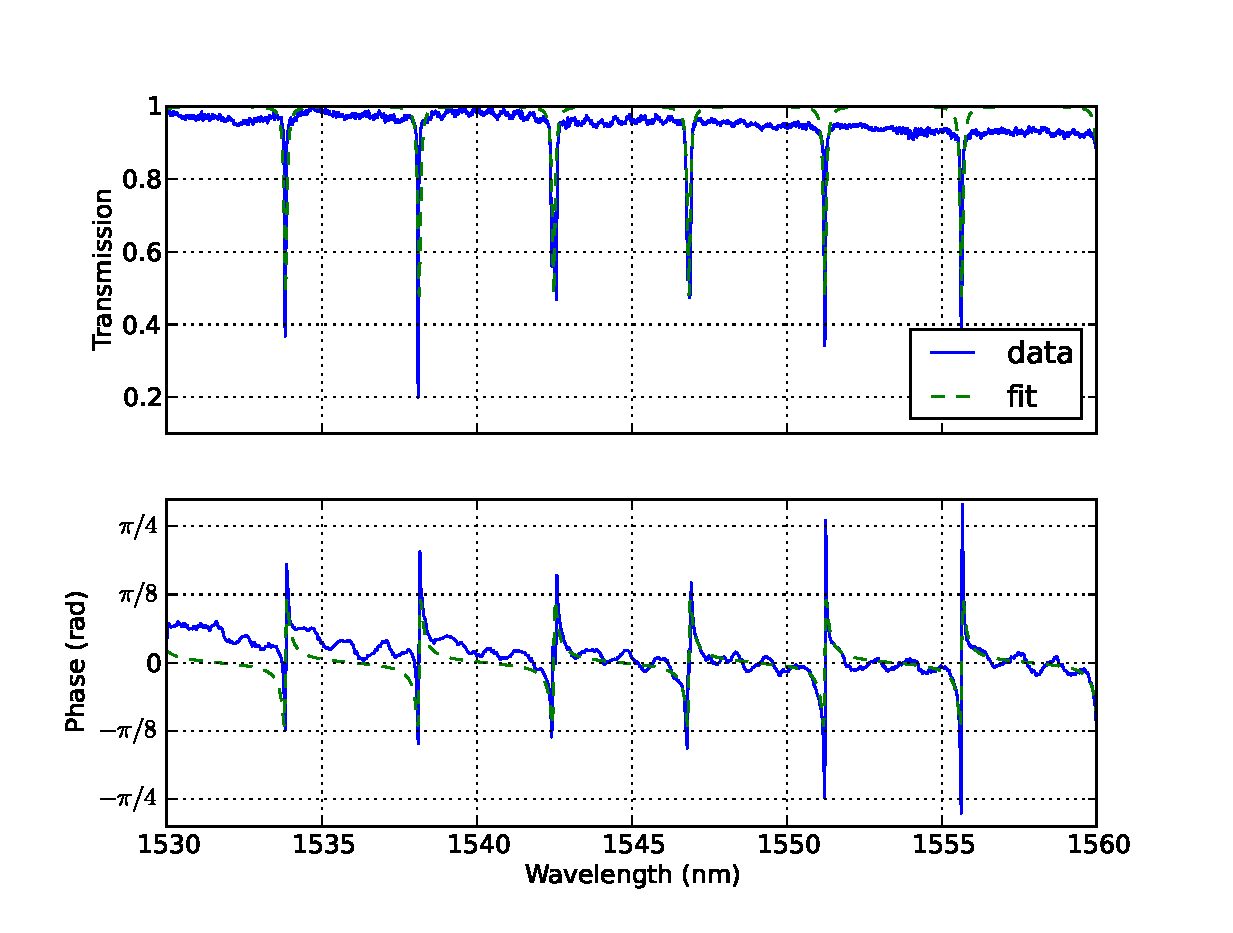
\includegraphics[width=9cm]{r20g275TE_fitPhaseAmp}}
  \caption{TE 20~$\mu$m radius and 275~nm gap ring spectrum measurement (--) and fit (-~-) for a coupling coefficient $k=0.22$, $\mathrm{losses=47~dB/cm}$ and effective index $n_{eff}=4.35$.}
  \label{fig:undercoupled} %[ k= 0.21659667  A= 0.93423178  neff= 4.35316758] -47.022906404 dB/cm
\end{figure}




\begin{figure}[htb]
  \centerline{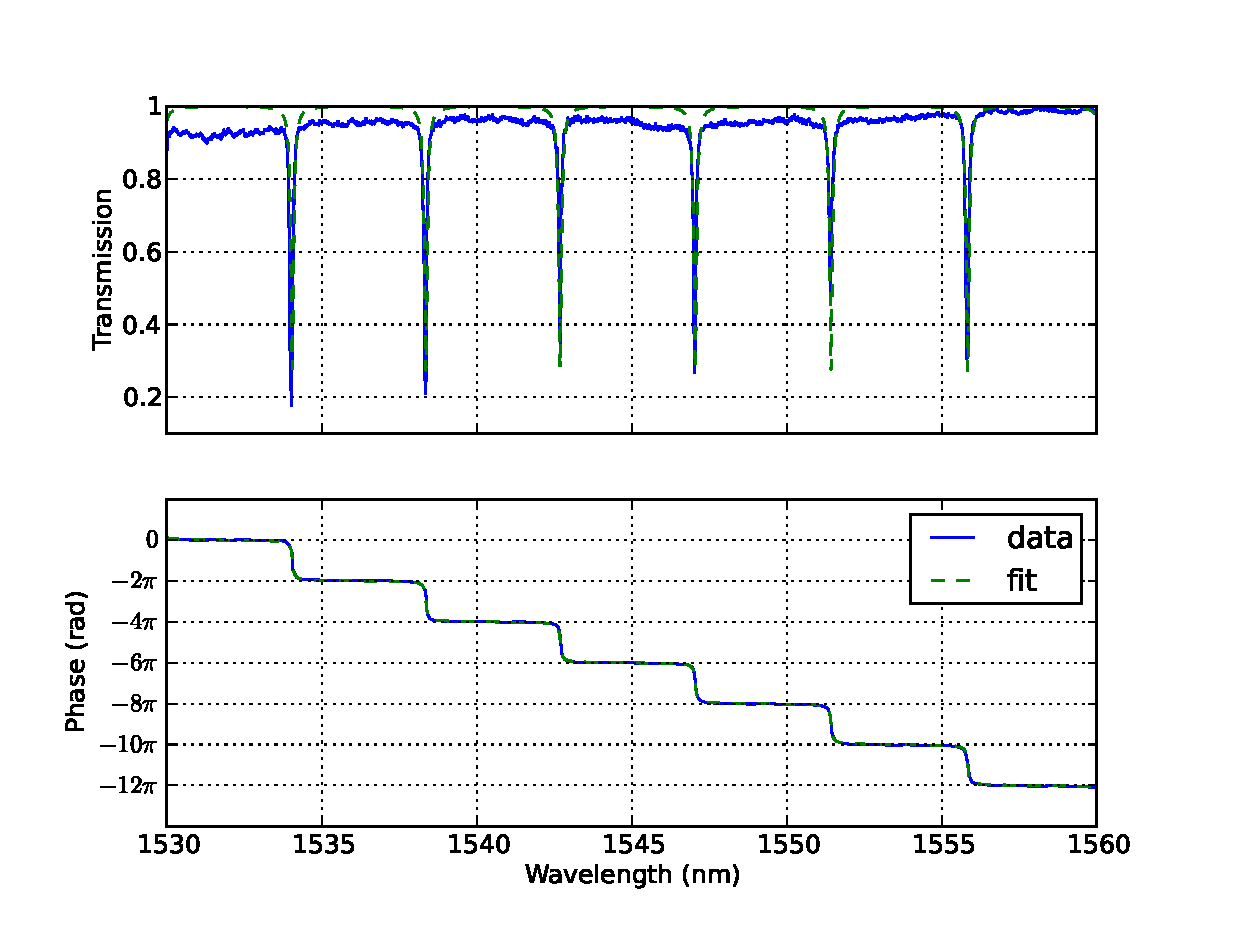
\includegraphics[width=9cm]{r20g200TE_fitPhaseAmp}}
  \caption{TE 20~$\mu$m radius and 200~nm gap ring spectrum measurement (--) and fit (-~-) for a coupling coefficient $k=0.35$, $\mathrm{losses=25~dB/cm}$ and effective index $n_{eff}=4.36$}
  \label{fig:overcoupled} % [k = 0.35048909  0.96328564  4.35909895] -25.8545799362 dB/cm
\end{figure}



\section{Slow light corrugated waveguides}
\label{sec:corrWaveguides}
The corrugated waveguides were designed with a nearly constant group index in a relatively broad wavelength range (from 1560 to 1610~nm), achievable by patterning circular holes onto the wide section of the waveguide as in~\cite{Brimont2010} (See Fig.~\ref{fig:sem}).
%Transverse-electric polarization (TE) light was coupled through grating couplers.

\begin{figure}[htb]
	\centering
	\includegraphics[width=2.5in]{corrV70}	
	\caption{Corrugated waveguide SEM image.}
	\label{fig:sem}
 \end{figure}


\subsection{Traditional group delay discrete measurement}
\label{sec:oldTechnique}
Traditional group delay measurements are based on fringe separation ~\cite{shang81,vlasov:05,yao:811,Dulkeith2006} and path balancing~\cite{Cohen:82,Knox:88,Liang:98} of a Mach-Zehnder interferometer.

% or very short pulses time-of-flight delay measurements~\cite{Vlasov:99}.

% In both cases the measurement is discrete and the resolution is limited by the path difference between branches.

% Paper~\cite{Dulkeith2006} determines group index and group velocity dispersion (GVD) of photonic wires by employing an integrated Mach-Zehnder interferometer

% In \cite{Dulkeith2006} dispersion and group index is characterized both for TE and TM waveguides. It is measured with an unbalanced integrated Mach Zehnder interferometer. So only a discrete amount of points is obtained, deriving group index and dispersion from them. On the other hand, our technique using a phase sensitive setup allows a more accurate continuous measurement with as high resolution as necessary.

In Fig.~\ref{fig:groupIndex} we show the fringes of an interferometer with a 450~$\mu$m corrugated waveguide in one branch and a reference photonic wire on the other branch. From the wavelength fringe separation ($ \lambda_{min} - \lambda_{max} $) we obtain the variation of the group delay with respect to the photonic wire $ n_{g,ref} $~\cite{vlasov:05}:

% Obtaining the differential group delay measurement from the variation of the fringes wavelength separation ($\Delta\lambda$):

% \begin{equation}
%   n_g (\lambda)=\frac{\lambda_0^2}{ L (\Delta\lambda)} + n_{g,ref}
% \end{equation}

\begin{equation}
  n_g (\lambda)=\frac{\lambda_{min} \lambda_{max}}{ 2L (\lambda_{min} - \lambda_{max})} + n_{g,ref}
\end{equation}


where $n_{g,ref}$ is the group index of the photonic wire obtained from the free spectral range (FSR) of the rings resonators in section~\ref{sec:ringResonators} (Eq.~\ref{eq:FSRanillo}).  %, $n_{g,ref}=4.36$

% With the variation between the separation of the fringes we can obtain the group index difference between the corrugated and the photonic wire:


% \begin{equation}
%   \Delta\lambda=\frac{\lambda_0^2}{n_g L}
% \end{equation}
% where $\Delta\lambda$ is the fringes separation, $n_g$ the group index and $\lambda_0$ is the central wavelength. The group index of the strip waveguide on the other branch was obtained from the free spectral range (FSR) of the rings resonators in section~\ref{sec:ringResonators} (Eq.~\ref{eq:FSRanillo}).  %, $n_{g,ref}=4.36$


\subsection{Proposed group delay continuous measurement}
\label{sec:newTechnique}
On the other hand, our technique provides a continuous phase characterization from which we can extract group delay with high resolution only limited by the laser step size.

We characterized and subtracted the phase evolutions of a 450~$\mu$m and a 27~$\mu$m corrugated waveguide to obtain the phase evolution of a 423~$\mu$m waveguide without the system response. To equalize our interferometer from the short (27~$\mu$m) to the long (450~$\mu$m) waveguide, a 11~ps delay increment was necessary in the optical-delay-line (ODL). This means that an equivalent $L=423~\mu$m-long corrugated waveguide has a group delay $T_g=11$~ps, which corresponds to a group index $n_g(\omega_0)=7.8$ (Eq.~\ref{eq:group_index_pathBalancing}). With the interferometer equalized we obtained the group index variations around $n_g(\omega_0)$ from the phase evolution differential~(Fig.~\ref{fig:groupIndex}).

% \begin{equation}
% 	\Delta \phi = \frac{d}{d\omega}(\phi_{long}-\phi_{short})=   L \frac{n_g(\omega)}{c}-11~ps+L\beta_2\Delta \omega + \ldots
% \end{equation}

% \begin{equation}
% 	\Delta \phi = \phi_{l}-\phi_{s}= L \beta_0 + \overbrace{ (L\beta_1-\frac{L_a}{c})\Delta \omega }+\frac{L}{2!}\beta_2\Delta \omega^2 + \ldots)
% \end{equation}


% \begin{equation}
%   \phi (\omega) = \phi _0 + (n_g(\omega)-n_{g}(\omega_0))(\omega-\omega_0) L+\frac{1}{2}\beta_2(\omega-\omega_0)^2 L+\ldots
% \end{equation}

% We characterized and subtracted the phase evolutions of a 450~$\mu$m and a 27~$\mu$m corrugated waveguide to obtain the phase evolution of a 423~$\mu$m waveguide without the system response. To equalize our interferometer from the short (27~$\mu$m) to the long (450~$\mu$m) waveguide, a 11~ps delay increment was necessary in the optical-delay-line (ODL). This means that an equivalent $L=423~\mu$m-long corrugated waveguide has a group delay $T_g=11$~ps, which corresponds to a group index $n_g=7.8$ (Eq.~\ref{eq:group_index_pathBalancing}). With the interferometer equalized we obtained the group index variations around $n_g=7.8$ (Fig.~\ref{fig:groupIndex}) from the first Taylor coefficient of the phase evolution ~\cite{shang81}:


% using coefficient $\beta_1=n_g/c$ of the propagation constant extracted from the phase measurements.
%of the $423~\mu$m.

% After re-equalizing the optical-delay-line (ODL)
% 
% As we had re-equalized the optical-delay-line (ODL) from the phase evolution we only obtained the group index variations around $n_g=7.8$ (See Fig.~\ref{fig:groupIndex})
% As we re-equalized both branches in the setup delaying in the ODL the group delay ($T_g$), we obtain group index variations with the differentiation of the phase evolution, obtaining the group index evolution shown in Fig.~\ref{fig:groupIndex}.


\begin{figure}[htb]
  \centering
  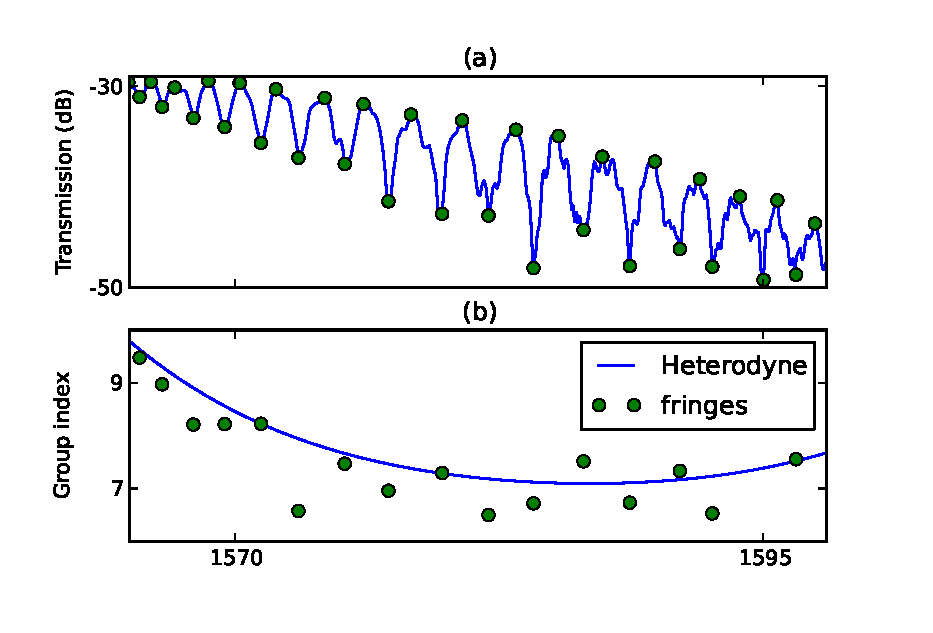
\includegraphics[width=3.5in]{gropIndexComparison_2}
  \caption{In blue line: continuous group index measurement. In green dots, traditional group index measurement using an indirect measurement of the phase with the fringes of a MZI interferometer. Fringes get closer at the band edges of the corrugated waveguide, known as slow light region, where we observe higher group index ($n_g$).} %(See section \ref{sec:oldTechnique})
  \label{fig:groupIndex}
\end{figure}



\section{Conclusion}
We have shown an experimental technique for phase response characterization of integrated photonic components. The technique cancels out phase noise by using a counter-propagating reference beam, thus avoiding the need of extremely fast tuning rates or cumbersome temperature control schemes. Two components, a microring resonator and a corrugated waveguide were characterized as examples of application. From the ring resonator results, overcoupling and undercoupling regimes were clearly distinguished from the phase response and excellent agreement with simulations was observed. In the corrugated waveguide, the group index profile in the slow-light band was measured with better resolution than with a traditional fringe-spacing method.


\section*{Acknowledgments}
We acknowledge financial support from the Spanish Ministry of Science and Innovation through contracts SINADEC (TEC2008- 06333) and PROMETEO/2010/087 NANOFOTONICA. Joaquin Matres is supported by a doctoral grant of the Universidad Polit\'ecnica de Valencia. We also acknowledge Binbin Guan for fruitful discussions and Jose Angel Ayucar for the his help taking the SEM pictures.

\begin{thebibliography}{10}
\providecommand{\url}[1]{#1}
\csname url@samestyle\endcsname
\providecommand{\newblock}{\relax}
\providecommand{\bibinfo}[2]{#2}
\providecommand{\BIBentrySTDinterwordspacing}{\spaceskip=0pt\relax}
\providecommand{\BIBentryALTinterwordstretchfactor}{4}
\providecommand{\BIBentryALTinterwordspacing}{\spaceskip=\fontdimen2\font plus
\BIBentryALTinterwordstretchfactor\fontdimen3\font minus
  \fontdimen4\font\relax}
\providecommand{\BIBforeignlanguage}[2]{{%
\expandafter\ifx\csname l@#1\endcsname\relax
\typeout{** WARNING: IEEEtran.bst: No hyphenation pattern has been}%
\typeout{** loaded for the language `#1'. Using the pattern for}%
\typeout{** the default language instead.}%
\else
\language=\csname l@#1\endcsname
\fi
#2}}
\providecommand{\BIBdecl}{\relax}
\BIBdecl

\bibitem{Vanwiggeren2003}
\BIBentryALTinterwordspacing
G.~D. VanWiggeren, A.~R. Motamedi, and D.~M. Barley, ``{Single-scan
  interferometric component analyzer},'' \emph{Photonics Technology Letters,
  IEEE}, vol.~15, no.~2, pp. 263--265, 2003. [Online]. Available:
  \url{http://ieeexplore.ieee.org/xpls/abs\_all.jsp?arnumber=1174140}
\BIBentrySTDinterwordspacing

\bibitem{Gifford2005}
D.~K. Gifford, B.~J. Soller, M.~S. Wolfe, and M.~E. Froggatt, ``{Optical vector
  network analyzer for single-scan measurements of loss, group delay, and
  polarization mode dispersion},'' \emph{Applied optics}, vol.~44, no.~34, pp.
  7282--7286, 2005.

\bibitem{Mas2012}
S.~Mas, J.~Matres, J.~Marti, C.~J. Oton, and J.~Mart\'{\i}, ``{Accurate
  chromatic dispersion characterization of photonic integrated circuits},''
  \emph{Photonics Journal, IEEE}, vol.~4, no.~3, pp. 825--831, Jun. 2012.

\bibitem{McKinnon2009}
\BIBentryALTinterwordspacing
W.~R. McKinnon, D.~X. Xu, C.~Storey, E.~Post, a.~Densmore, a.~Del\^{a}ge,
  P.~Waldron, J.~H. Schmid, and S.~Janz, ``{Extracting coupling and loss
  coefficients from a ring resonator.}'' \emph{Optics express}, vol.~17,
  no.~21, pp. 18\,971--82, Oct. 2009. [Online]. Available:
  \url{http://www.ncbi.nlm.nih.gov/pubmed/20372631}
\BIBentrySTDinterwordspacing

\bibitem{Brimont2010}
\BIBentryALTinterwordspacing
A.~Brimont, J.~V. Gal\'{a}n, J.~M. Escalante, J.~Mart\'{\i}, and P.~Sanchis,
  ``{Group-index engineering in silicon corrugated waveguides.}'' \emph{Optics
  letters}, vol.~35, no.~16, pp. 2708--10, Aug. 2010. [Online]. Available:
  \url{http://www.ncbi.nlm.nih.gov/pubmed/20717431}
\BIBentrySTDinterwordspacing

\bibitem{shang81}
H.-T. Shang, ``{Chromatic dispersion measurement by white-light interferometry
  on metre-length single-mode optical fibres},'' \emph{Electronics Letters},
  vol.~17, no.~17, pp. 603--605, 1981.

\bibitem{vlasov:05}
Y.~A. Vlasov, M.~O'Boyle, H.~F. Hamann, and S.~J. McNab, ``{Active control of
  slow light on a chip with photonic crystal waveguides},'' \emph{Nature}, vol.
  438, no. 7064, pp. 65--69, 2005.

\bibitem{yao:811}
\BIBentryALTinterwordspacing
X.~S. Yao and J.~Feinberg, ``{Simple in-line method to measure the dispersion
  of an optical system},'' \emph{Applied Physics Letters}, vol.~62, no.~8, pp.
  811--813, 1993. [Online]. Available:
  \url{http://link.aip.org/link/?APL/62/811/1}
\BIBentrySTDinterwordspacing

\bibitem{Dulkeith2006}
\BIBentryALTinterwordspacing
E.~Dulkeith, F.~Xia, L.~Schares, W.~M.~J. Green, L.~Sekaric, and Y.~A. Vlasov,
  ``{Group index and group velocity dispersion in silicon-on-insulator photonic
  wires.}'' \emph{Optics express}, vol.~14, no.~13, p. 6372, Jun. 2006.
  [Online]. Available:
  \url{http://www.opticsinfobase.org/abstract.cfm?\&amp;id=89589
  http://www.ncbi.nlm.nih.gov/pubmed/19516814}
\BIBentrySTDinterwordspacing

\bibitem{Cohen:82}
L.~G. Cohen and J.~Stone, ``{Interferometric measurements of minimum dispersion
  spectra in short lengths of single-mode fibre},'' \emph{Electronics Letters},
  vol.~18, no.~13, pp. 564--566, 1982.

\bibitem{Knox:88}
\BIBentryALTinterwordspacing
W.~H. Knox, N.~M. Pearson, K.~D. Li, and C.~A. Hirlimann, ``{Interferometric
  measurements of femtosecond group delay in optical components},'' \emph{Opt.
  Lett.}, vol.~13, no.~7, pp. 574--576, Jul. 1988. [Online]. Available:
  \url{http://ol.osa.org/abstract.cfm?URI=ol-13-7-574}
\BIBentrySTDinterwordspacing

\bibitem{Liang:98}
\BIBentryALTinterwordspacing
Y.~Liang and C.~P. Grover, ``{Modified white-light Mach-Zehnder interferometer
  for direct group-delay measurements},'' \emph{Appl. Opt.}, vol.~37, no.~19,
  pp. 4105--4111, Jul. 1998. [Online]. Available:
  \url{http://ao.osa.org/abstract.cfm?URI=ao-37-19-4105}
\BIBentrySTDinterwordspacing

\end{thebibliography}

%\bibliographystyle{IEEEtran}
%\bibliography{/home/joaquin/Documents/library}
\end{document}

